%! Author = jdubec
%! Date = 16/02/2026

\documentclass[11pt, a4paper]{article}

% ─── Packages ────────────────────────────────────────────────────────────────
\usepackage[utf8]{inputenc}
\usepackage[T1]{fontenc}
\usepackage[margin=2.5cm]{geometry}
\usepackage{graphicx}
\usepackage{hyperref}
\usepackage{booktabs}
\usepackage{float}
\usepackage{xcolor}
\usepackage{listings}
\hypersetup{colorlinks=true, linkcolor=black, citecolor=black, urlcolor=blue!70!black}

% ─── Code listing style ─────────────────────────────────────────────────────
\lstset{
    basicstyle=\ttfamily\small,
    breaklines=true,
    frame=single,
    numbers=left,
    numberstyle=\tiny\color{gray},
    xleftmargin=2em,
    framexleftmargin=1.5em
}

% ─── Bibliography ────────────────────────────────────────────────────────────
\usepackage[style=numeric, backend=bibtex]{biblatex}
\addbibresource{references.bib}

% ─── Language ────────────────────────────────────────────────────────────────
\input{lang/en}

% ─── Student details ─────────────────────────────────────────────────────────
\newcommand{\StudentName}{Matej Straka, Michal Novick\'{y}}
\newcommand{\StudyGroup}{Thursday 9:00}
\newcommand{\AssignmentNumber}{3}
\newcommand{\AssignmentTitle}{Filmov\'{y} port\'{a}l}
\newcommand{\AcademicYear}{2025/2026}

% =============================================================================
\begin{document}

% ─── Cover page ──────────────────────────────────────────────────────────────
\begin{titlepage}
    \centering

    \includegraphics[width=0.3\textwidth]{../assets/logo}

    \vspace{0.3cm}
    {\large \LabelUniversity}\\[2pt]
    {\large \LabelFaculty}

    \vspace{2.5cm}
    {\Huge\bfseries \LabelProtocol}

    \vspace{0.6cm}
    {\LARGE \LabelCode{} --- \LabelCourse}

    \vspace{0.4cm}
    {\Large \LabelAssignment{} \AssignmentNumber: \AssignmentTitle}

    \vfill

    \begin{tabular}{r l}
        \textbf{\LabelStudent:} & \StudentName  \\[4pt]
        \textbf{\LabelGroup:}   & \StudyGroup   \\[4pt]
        \textbf{\LabelYear:}    & \AcademicYear \\[4pt]
        \textbf{\LabelDate:}    & \today        \\
    \end{tabular}

    \vspace{1.5cm}
\end{titlepage}

% ─── Table of contents ───────────────────────────────────────────────────────
\renewcommand{\contentsname}{\LabelContents}
\tableofcontents
\newpage

% =============================================================================

% ─────────────────────────────────────────────────────────────────────────────
\section{Changes from Assignment 1}
\label{sec:changes}
% ─────────────────────────────────────────────────────────────────────────────

The core data model from Assignment~1 remained stable. Two targeted changes
were made during physical implementation after discovering minor gaps in the
original design.

\subsection{Added \texttt{added\_at} to \texttt{watchlists\_movies}}

\noindent\textbf{Change:} A column \texttt{added\_at TIMESTAMP NOT NULL
DEFAULT CURRENT\_TIMESTAMP} was added to the \texttt{watchlists\_movies}
junction table.

\noindent\textbf{Reason:} The original design treated this table as a pure
many-to-many bridge with no additional attributes. During implementation it
became clear that recording \emph{when} a movie was added to a watchlist is
useful both for ordering items within a list (``recently added first'') and
for analytical queries about watchlist activity over time. This pattern is
standard in production watchlist systems.

\subsection{Added \texttt{role} column to \texttt{watchlists\_users}}

\noindent\textbf{Change:} The \texttt{watchlists\_users} junction table
gained a \texttt{role watchlist\_user\_role\_enum NOT NULL DEFAULT
'follower'} column. The ENUM type defines three values:
\texttt{'owner'}, \texttt{'editor'}, and \texttt{'follower'}.

\noindent\textbf{Reason:} Assignment~1 described watchlists as shareable
but did not differentiate user roles within a shared list. The physical
model needed a way to distinguish the creator (owner), collaborators who can
modify the list (editors), and passive subscribers (followers). Using an
ENUM type keeps the constraint self-documenting and prevents invalid role
strings at the database level.

\noindent The updated physical model diagram is shown in
Figure~\ref{fig:model}.

% ─────────────────────────────────────────────────────────────────────────────
\newpage
\section{Physical Model --- Implementation}
\label{sec:physical}
% ─────────────────────────────────────────────────────────────────────────────

\subsection{Table overview}

\begin{table}[H]
    \centering
    \caption{Tables in the film portal database}
    \label{tab:tables}
    \begin{tabular}{l p{9cm}}
        \toprule
        \textbf{Table} & \textbf{Description} \\
        \midrule
        \texttt{users}
            & Registered accounts; stores credentials, display name, and
              role (\texttt{user} / \texttt{admin}). \\
        \texttt{movies}
            & Central catalogue entry: title, release year, runtime, and
              pre-aggregated rating statistics. \\
        \texttt{people}
            & Directors, actors, and writers referenced by
              \texttt{movies\_people}. \\
        \texttt{genres}
            & Lookup table of genre labels; enforces consistent
              categorisation. \\
        \texttt{ratings}
            & Numerical score (0--10) submitted by one user for one movie. \\
        \texttt{reviews}
            & Free-text review (min.\ 50 characters) by one user for one
              movie. \\
        \texttt{watchlists}
            & Named, optionally public collection of movies. \\
        \texttt{movies\_genres}
            & M:N bridge between movies and genres. \\
        \texttt{movies\_people}
            & M:N bridge between movies and people; includes a role
              attribute (\texttt{actor} / \texttt{director} /
              \texttt{writer}). \\
        \texttt{watchlists\_users}
            & M:N bridge between watchlists and users; includes a role
              attribute (\texttt{owner} / \texttt{editor} /
              \texttt{follower}). \\
        \texttt{watchlists\_movies}
            & M:N bridge between watchlists and movies; records the
              timestamp when each movie was added. \\
        \bottomrule
    \end{tabular}
\end{table}

\subsection{Notable integrity constraints}

The constraints below protect non-trivial business rules that go beyond
simple NOT NULL checks.

\begin{itemize}
    \item \textbf{Rating and review uniqueness ---}
    \texttt{UNIQUE (user\_id, movie\_id)} in both \texttt{ratings} and
    \texttt{reviews} ensures one score and one review per user per film.
    This prevents score manipulation and duplicate content at the database
    level, regardless of the application layer.

    \item \textbf{Movie uniqueness ---}
    \texttt{UNIQUE (title, release\_year)} in \texttt{movies} blocks exact
    duplicates while permitting legitimate remakes released in different
    years.

    \item \textbf{Realistic release year ---}
    \texttt{CHECK (release\_year BETWEEN 1888 AND 2040)} bounds entries to
    the era of cinema (first known film: 1888) and allows pre-announced
    near-future releases.

    \item \textbf{Score range ---}
    \texttt{CHECK (score BETWEEN 0 AND 10)} in \texttt{ratings} and
    \texttt{CHECK (average\_rating BETWEEN 0 AND 10)} in \texttt{movies}
    guarantee that every displayed score lies within the expected scale.

    \item \textbf{Minimum review length ---}
    \texttt{CHECK (LENGTH(content) >= 50)} in \texttt{reviews} prevents
    one-word spam at the storage level and enforces a basic quality floor.

    \item \textbf{Composite role key in \texttt{movies\_people} ---}
    The primary key \texttt{(movie\_id, person\_id, role)} allows the same
    person to be listed as both director and actor in one film, while
    blocking the same role being assigned twice.

    \item \textbf{Watchlist user role ---}
    \texttt{role watchlist\_user\_role\_enum NOT NULL DEFAULT 'follower'}
    in \texttt{watchlists\_users} restricts membership roles to the three
    defined values, with a safe default for newly followed lists.
\end{itemize}

\subsection{ON DELETE strategies}

All foreign keys in the schema use \texttt{ON DELETE CASCADE}. The
governing principle is that every dependent row derives its meaning
entirely from its parent: a rating without a user or movie is orphaned
data, a genre link without a movie is meaningless, and so on. Cascading
deletes prevent constraint violations during administrative bulk operations
(e.g.\ removing a duplicate movie entry) and keep the database
self-consistent without requiring application-side cleanup logic.

\texttt{RESTRICT} was considered for genre and person deletions to force
explicit confirmation before removing shared lookup data, but
\texttt{CASCADE} was chosen for uniformity and operational safety during
data corrections.

% ─────────────────────────────────────────────────────────────────────────────
\newpage
\section{Seed Data}
\label{sec:seed}
% ─────────────────────────────────────────────────────────────────────────────

\subsection{Generation approach}

Seed data was generated using a Python script (\texttt{seed/seed.py}) with
the \textbf{Faker} library for realistic names, usernames, review text, and
descriptions, and the \textbf{bcrypt} library for password hashing. All rows
are emitted as plain SQL \texttt{INSERT} statements into a single
\texttt{seed.sql} file, wrapped in one transaction (\texttt{BEGIN} /
\texttt{COMMIT}). A fixed random seed (\texttt{SEED = 42}, applied to both
\texttt{random} and \texttt{Faker}) guarantees that re-running the script
produces identical output. Running instructions are provided in
\texttt{seed/README.md}.

\subsection{Record counts after seeding}

\begin{table}[H]
    \centering
    \caption{Row counts per table after seeding}
    \label{tab:seed-counts}
    \begin{tabular}{l r}
        \toprule
        \textbf{Table} & \textbf{Row count} \\
        \midrule
        \texttt{genres}              & 20     \\
        \texttt{users}               & 1\,000 \\
        \texttt{people}              & 1\,000 \\
        \texttt{movies}              & 500    \\
        \texttt{movies\_genres}      & $\approx$1\,000 \\
        \texttt{movies\_people}      & $\approx$4\,750 \\
        \texttt{ratings}             & 6\,000 \\
        \texttt{reviews}             & 2\,000 \\
        \texttt{watchlists}          & 500    \\
        \texttt{watchlists\_users}   & $\approx$1\,200 \\
        \texttt{watchlists\_movies}  & $\approx$17\,000 \\
        \midrule
        \textbf{Total}               & $\mathbf{>34\,000}$ \\
        \bottomrule
    \end{tabular}
\end{table}

\noindent Row counts marked with $\approx$ vary slightly between runs due to
weighted random sampling; all other counts are exact.

\subsection{Distribution strategy}

The distribution is intentionally non-uniform to reflect realistic usage
patterns.

\begin{itemize}
    \item \textbf{Ratings --- streak users:} 50 users were randomly selected
    to generate 1--3 consecutive-day rating streaks of 4--30 days each,
    with ratings placed in the evening hours (18:00--23:59). This ensures
    the streak analytical query (Process~2) has meaningful data to work
    with. The remaining ratings up to the target of 6\,000 are distributed
    uniformly across all users and movies.

    \item \textbf{Rating scores:} Scores are drawn from a weighted
    distribution that favours mid-to-high values
    (weights 1, 1, 2, 3, 5, 8, 12, 16, 18, 16, 10 for scores 0--10),
    matching the positive-skew pattern typical of voluntary rating systems
    where users tend to rate movies they already liked.

    \item \textbf{Reviews:} Only (user, movie) pairs that already have a
    rating are eligible for a review. 2\,000 such pairs are sampled
    uniformly, reflecting the real-world behaviour where reviews are far
    less common than numerical scores.

    \item \textbf{Watchlist sizes:} Each watchlist receives 1--67 movies
    sampled uniformly, which produces a right-skewed distribution. Sharing
    is weighted so that 20\% of watchlists are private (not shared beyond
    the owner) and the rest have 1--4 additional members; follower roles
    are roughly twice as common as editor roles.

    \item \textbf{Movie genres and cast:} Each movie receives 1--3 genres
    (weighted 40/45/15\%) and a variable cast: 1--2 directors, 1--3
    writers, and 3--8 actors, all sampled without replacement from the
    people pool.

    \item \textbf{User roles:} The first 10 users (by insertion order) are
    assigned the \texttt{admin} role; all remaining 990 users receive the
    default \texttt{user} role.
\end{itemize}

\subsection{Consistency guarantees}

\begin{itemize}
    \item Rows are inserted in strict dependency order: genres, users, people,
    movies, then all junction and fact tables. PostgreSQL enforces foreign key
    constraints on every insert, so any ordering error surfaces immediately.

    \item The \texttt{UNIQUE (user\_id, movie\_id)} constraint on
    \texttt{ratings} is respected during generation: a \texttt{rating\_pairs}
    set tracks all assigned pairs and duplicate candidates are resampled
    before insertion.

    \item The \texttt{average\_rating}, \texttt{total\_ratings}, and
    \texttt{total\_reviews} columns in \texttt{movies} are computed in-memory
    after all ratings and reviews are generated, then written into the
    \texttt{INSERT} statements for \texttt{movies} --- so the pre-aggregated
    values are always consistent with the inserted fact rows.

    \item All timestamps (\texttt{created\_at}, \texttt{added\_at}) fall
    within the range 2026-01-01 to 2026-05-31, which is a realistic
    operational window and avoids \texttt{CHECK} violations on
    \texttt{birth\_year} or \texttt{release\_year}.
\end{itemize}

% ─────────────────────────────────────────────────────────────────────────────
\newpage
\section{Process 1 --- Rating a Movie}
\label{sec:process1}
% ─────────────────────────────────────────────────────────────────────────────

% TODO: Fill in after process SQL is finalised and approved by the instructor.
%
% Required subsections per assignment specification:
%   \subsection{Process description and link to use case}
%   \subsection{SQL implementation}      -- full query + any views
%   \subsection{Sample execution}        -- input params + first 10 rows of output
%   \subsection{Correctness verification}
%   \subsection{Indexes supporting this process}

\textit{[To be completed after instructor approval of selected processes.]}

% ─────────────────────────────────────────────────────────────────────────────
\newpage
\section{Process 2 --- User Rating Streak}
\label{sec:process2}
% ─────────────────────────────────────────────────────────────────────────────

\subsection{Process description and link to use case}

This is an \textbf{analytical process} corresponding to the reporting
perspective of the ``Searching and filtering movies'' use case from
Assignment~1: identifying the most active rating periods across all users.

The query finds every \textbf{consecutive-day rating streak} for every
user. A streak is a maximal sequence of calendar days on which a user
submitted at least one rating, with no gap larger than one day between
any two consecutive active days. For each qualifying streak the query
reports:

\begin{itemize}
    \item the user's full name,
    \item the start and end date of the streak,
    \item the total length of the streak in calendar days,
    \item the number of movies rated during the streak,
    \item the average score given during the streak.
\end{itemize}

Only streaks of \textbf{at least 5 consecutive days} are returned,
ordered by length (longest first), then by end date (most recent first).

\begin{itemize}
    \item \textbf{Input:} None --- the query runs over the full
    \texttt{ratings} table.
    \item \textbf{Output:} One row per qualifying streak with the columns
    listed above.
\end{itemize}

\subsection{SQL implementation}

The full query is provided in \texttt{queries.sql}. It is built in three
nested layers, each building on the previous one.

\subsubsection{Query logic explained}

The query proceeds in three steps:

\begin{enumerate}
    \item \textbf{Innermost subquery (alias \texttt{z}):}
    For each rating row, \texttt{LAG(created\_at)} fetches the timestamp
    of the same user's previous rating, ordered chronologically.
    Both values are truncated to \texttt{DATE} so that multiple ratings
    on the same calendar day count as a single active day.
    The result is a flat table of
    \texttt{(user\_id, movie\_id, score, date, prev\_date)}.

    \item \textbf{Middle subquery (alias \texttt{x}):}
    A running \texttt{SUM} window function increments a
    \texttt{group\_id} counter each time the gap between two consecutive
    rating dates for the same user exceeds one calendar day.
    Because the counter only increases on gaps, all rows within an
    uninterrupted streak share the same \texttt{group\_id} value.
    The \texttt{movies} table is joined here to carry the film title.

    \item \textbf{Outer query:}
    Rows are grouped by \texttt{(user\_id, group\_id)}, which uniquely
    identifies one streak for one user. Aggregate functions compute the
    streak start and end dates, the calendar length, the number of
    ratings, and the average score. A \texttt{WHERE} clause keeps only
    streaks of at least 5 days, and results are sorted as required.
\end{enumerate}

\subsection{Sample execution on seed data}

% TODO: Once seed data is loaded, run the query and paste the first
% 10 rows here as a table. Example format:
%
% \begin{table}[H]
%   \centering
%   \caption{First 10 rows returned by the rating streak query (seed data)}
%   \label{tab:streak-sample}
%   \begin{tabular}{l c c r r r}
%     \toprule
%     \textbf{name} & \textbf{start\_date} & \textbf{end\_date}
%       & \textbf{days} & \textbf{movies} & \textbf{avg} \\
%     \midrule
%     ... & ... & ... & ... & ... & ... \\
%     \bottomrule
%   \end{tabular}
% \end{table}

\textit{[To be completed after seed data is loaded.]}

\subsection{Correctness verification}

The correctness of the streak grouping was verified by:

\begin{enumerate}
    \item Manually tracing \texttt{group\_id} values for a single test
    user whose ratings were inserted on known consecutive and
    non-consecutive dates, confirming that each gap correctly increments
    the counter.
    \item Checking that \texttt{days\_streak = MAX(date) - MIN(date) + 1}
    matches the expected calendar span for each identified streak group.
    \item Confirming that the \texttt{UNIQUE (user\_id, movie\_id)}
    constraint on \texttt{ratings} guarantees each movie appears at most
    once per user, so \texttt{COUNT(*)} equals the number of distinct
    movies rated within the streak.
\end{enumerate}

\subsection{Indexes supporting this process}

% TODO: Add index definitions and justifications here.
% Minimum recommended for this process:
%   - ratings(user_id)               -- speeds up PARTITION BY user_id
%   - ratings(user_id, created_at)   -- composite; eliminates sort for LAG window
%   - ratings(created_at)            -- supports range scans on date filters
%
% Include EXPLAIN (ANALYZE, BUFFERS) before/after at least one index
% in Section~\ref{sec:performance}.

\textit{[To be completed together with Section~\ref{sec:performance}.]}

% ─────────────────────────────────────────────────────────────────────────────
\newpage
\section{Performance and Indexes --- Summary}
\label{sec:performance}
% ─────────────────────────────────────────────────────────────────────────────

% TODO: Fill in after index creation and EXPLAIN ANALYZE runs.
%
% Required content per assignment specification:
%   - Complete list of all created indexes (table, columns, type, purpose).
%   - At least one EXPLAIN (ANALYZE, BUFFERS) before/after comparison
%     with a short comment explaining what changed (e.g. Seq Scan ->
%     Index Scan, cost reduction, buffer hits, etc.).
%   - Note which queries remain slow even with indexes and why
%     (e.g. small table => planner prefers seq scan, high row estimate).

\textit{[To be completed after index creation and EXPLAIN ANALYZE
measurements.]}

% ─────────────────────────────────────────────────────────────────────────────
\newpage
\section{Evaluation}
\label{sec:evaluation}
% ─────────────────────────────────────────────────────────────────────────────

% TODO: Fill in at the end of the project.
%
% Required reflections per assignment specification:
%   - Which part surprised you most --- seed, queries, or indexes? Why?
%   - Did you discover a bug in the original model during implementation?
%     How did you fix it?
%   - Which business rule was hardest to express in pure SQL and why?
%   - Did you use AI tools? For what exactly, what was the raw output,
%     and how did you modify or verify it?

\textit{[To be completed at the end of the project.]}

% ─── Bibliography ────────────────────────────────────────────────────────────
\printbibliography

% ─── Attachments ─────────────────────────────────────────────────────────────
\newpage
\appendix

\section{Physical model diagram}
\label{sec:attachment-model}

\begin{figure}[H]
    \centering
    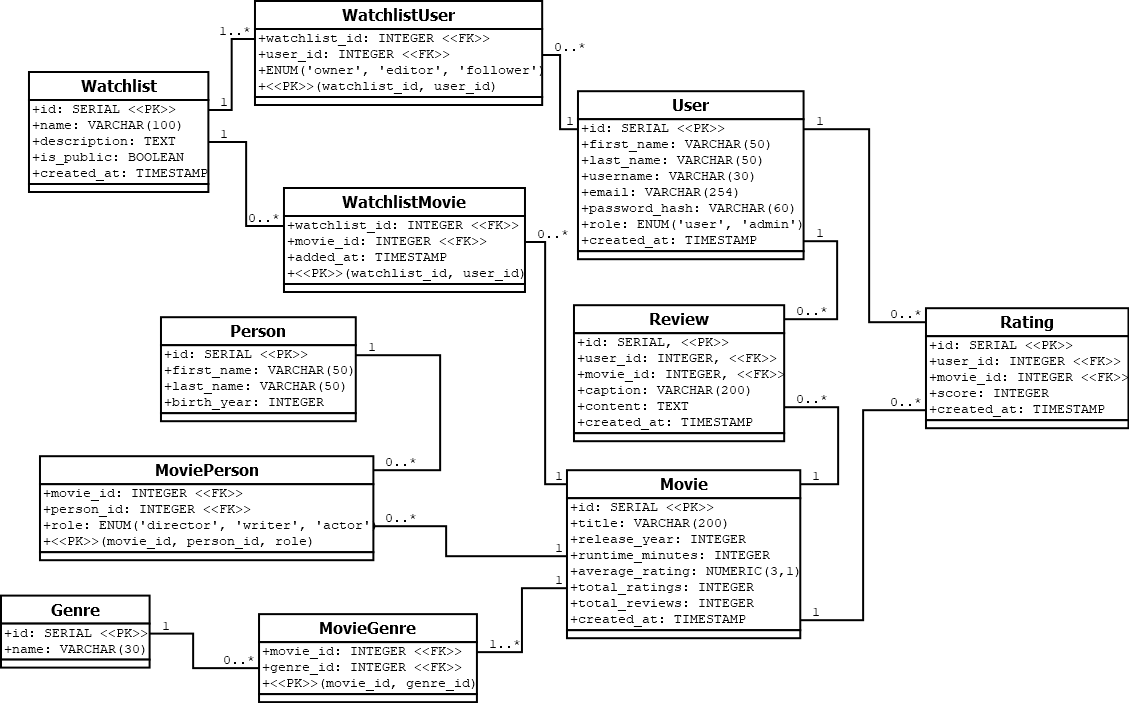
\includegraphics[width=\textwidth]{../assets/Model}
    \caption{Updated physical relational model --- Film portal}
    \label{fig:model}
\end{figure}

\end{document}
